% Options for packages loaded elsewhere
\PassOptionsToPackage{unicode}{hyperref}
\PassOptionsToPackage{hyphens}{url}
%
\documentclass[
  12pt,
]{article}
\usepackage{amsmath,amssymb}
\usepackage{lmodern}
\usepackage{iftex}
\ifPDFTeX
  \usepackage[T1]{fontenc}
  \usepackage[utf8]{inputenc}
  \usepackage{textcomp} % provide euro and other symbols
\else % if luatex or xetex
  \usepackage{unicode-math}
  \defaultfontfeatures{Scale=MatchLowercase}
  \defaultfontfeatures[\rmfamily]{Ligatures=TeX,Scale=1}
\fi
% Use upquote if available, for straight quotes in verbatim environments
\IfFileExists{upquote.sty}{\usepackage{upquote}}{}
\IfFileExists{microtype.sty}{% use microtype if available
  \usepackage[]{microtype}
  \UseMicrotypeSet[protrusion]{basicmath} % disable protrusion for tt fonts
}{}
\makeatletter
\@ifundefined{KOMAClassName}{% if non-KOMA class
  \IfFileExists{parskip.sty}{%
    \usepackage{parskip}
  }{% else
    \setlength{\parindent}{0pt}
    \setlength{\parskip}{6pt plus 2pt minus 1pt}}
}{% if KOMA class
  \KOMAoptions{parskip=half}}
\makeatother
\usepackage{xcolor}
\IfFileExists{xurl.sty}{\usepackage{xurl}}{} % add URL line breaks if available
\IfFileExists{bookmark.sty}{\usepackage{bookmark}}{\usepackage{hyperref}}
\hypersetup{
  pdftitle={State-space age-structured assessment models provide reliable inferences(?)},
  pdfauthor={Timothy J. Miller1, Britten, Brooks, Fay, Legault, Stock,},
  hidelinks,
  pdfcreator={LaTeX via pandoc}}
\urlstyle{same} % disable monospaced font for URLs
\usepackage[margin=1in]{geometry}
\usepackage{graphicx}
\makeatletter
\def\maxwidth{\ifdim\Gin@nat@width>\linewidth\linewidth\else\Gin@nat@width\fi}
\def\maxheight{\ifdim\Gin@nat@height>\textheight\textheight\else\Gin@nat@height\fi}
\makeatother
% Scale images if necessary, so that they will not overflow the page
% margins by default, and it is still possible to overwrite the defaults
% using explicit options in \includegraphics[width, height, ...]{}
\setkeys{Gin}{width=\maxwidth,height=\maxheight,keepaspectratio}
% Set default figure placement to htbp
\makeatletter
\def\fps@figure{htbp}
\makeatother
\setlength{\emergencystretch}{3em} % prevent overfull lines
\providecommand{\tightlist}{%
  \setlength{\itemsep}{0pt}\setlength{\parskip}{0pt}}
\setcounter{secnumdepth}{5}
\newlength{\cslhangindent}
\setlength{\cslhangindent}{1.5em}
\newlength{\csllabelwidth}
\setlength{\csllabelwidth}{3em}
\newlength{\cslentryspacingunit} % times entry-spacing
\setlength{\cslentryspacingunit}{\parskip}
\newenvironment{CSLReferences}[2] % #1 hanging-ident, #2 entry spacing
 {% don't indent paragraphs
  \setlength{\parindent}{0pt}
  % turn on hanging indent if param 1 is 1
  \ifodd #1
  \let\oldpar\par
  \def\par{\hangindent=\cslhangindent\oldpar}
  \fi
  % set entry spacing
  \setlength{\parskip}{#2\cslentryspacingunit}
 }%
 {}
\usepackage{calc}
\newcommand{\CSLBlock}[1]{#1\hfill\break}
\newcommand{\CSLLeftMargin}[1]{\parbox[t]{\csllabelwidth}{#1}}
\newcommand{\CSLRightInline}[1]{\parbox[t]{\linewidth - \csllabelwidth}{#1}\break}
\newcommand{\CSLIndent}[1]{\hspace{\cslhangindent}#1}
\usepackage{url}
\usepackage{setspace}
%\singlespacing
%\onehalfspacing
\doublespacing
\usepackage{lineno}
\linenumbers
\usepackage[belowskip=0pt,aboveskip=0pt]{caption}
\usepackage{relsize}
\newcommand{\afrb}{Alaska Fishery Research Bulletin\xspace}
\newcommand{\ajms}{African Journal of Marine Science\xspace}
\newcommand{\amb}{Advances in Marine Biology\xspace}
\newcommand{\bms}{Bulletin of Marine Science\xspace}
\newcommand{\bjssf}{Bulletin of the Japanese Society of Scientific Fisheries\xspace}
\newcommand{\cb}{Conservation Biology\xspace}
\newcommand{\cjfas}{Canadian Journal of Fisheries and Aquatic Sciences\xspace}
\newcommand{\ea}{Ecological Applications\xspace}
\newcommand{\eer}{Evolutionary Ecology Research\xspace}
\newcommand{\elet}{Ecology Letters\xspace}
\newcommand{\emod}{Ecological Modelling\xspace}
\newcommand{\ebf}{Environmental Biology of Fishes\xspace}
\newcommand{\ff}{Fish and Fisheries\xspace}
\newcommand{\fo}{Fisheries Oceanography\xspace}
\newcommand{\fr}{Fisheries Research\xspace}
\newcommand{\fb}{Fishery Bulletin\xspace}
\newcommand{\ijms}{ICES Journal of Marine Science\xspace}
\newcommand{\iccat}{Collective Volume of Scientific Papers ICCAT\xspace}
\newcommand{\jae}{Journal of Animal Ecology\xspace}
\newcommand{\jai}{Journal of Applied Ichthyology\xspace}
\newcommand{\jdc}{Journal Du Conseil International Pour L'exploration De La Mer\xspace}
\newcommand{\jdcp}{Journal Du Conseil Permanent International Pour L'exploration De La Mer\xspace}
\newcommand{\jembe}{Journal of Experimental Marine Biology and Ecology\xspace}
\newcommand{\jfb}{Journal of Fish Biology\xspace}
\newcommand{\jsr}{Journal of Sea Research\xspace}
\newcommand{\jtb}{Journal of Theoretical Biology\xspace}
\newcommand{\jfrbc}{Journal of the Fisheries Research Board of Canada\xspace}
\newcommand{\jnwafs}{Journal of Northwest Atlantic Fisheries Science\xspace}
\newcommand{\mcf}{Marine and Coastal Fisheries: Dynamics, Management, and Ecosystem Science\xspace}
\newcommand{\mb}{Marine Biology\xspace}
\newcommand{\meps}{Marine Ecology Progress Series\xspace}
\newcommand{\mfr}{Marine Fisheries Review\xspace}
\newcommand{\mpb}{Marine Pollution Bulletin\xspace}
\newcommand{\najfm}{North American Journal of Fisheries Management\xspace}
\newcommand{\nzjmfr}{New Zealand Journal of Marine and Freshwater Research\xspace}
\newcommand{\pnas}{Proceedings of the National Academy of Sciences USA\xspace}
\newcommand{\rpvrciemm}{Rapports et Proc\`es-Verbaux des R\'eunions. Conseil Internationale pour l'Exploration de la Mer\xspace}
\newcommand{\rpvrcpiemm}{Rapports et Proc\`es-Verbaux des R\'eunions. Conseil Permanent Internationale pour l'Exploration de la Mer\xspace}
\newcommand{\rfbf}{Reviews in Fish Biology and Fisheries\xspace}
\newcommand{\sajms}{South African Journal of Marine Science\xspace}
\newcommand{\tafs}{Transactions of the American Fisheries Society\xspace}

\newcommand{\anzjs}{Australian \& New Zealand Journal of Statistics\xspace}
\newcommand{\as}{Applied Statistics\xspace}
\newcommand{\csda}{Computational Statistics \& Data Analysis\xspace}
\newcommand{\ees}{Environmental and Ecological Statistics\xspace}
\newcommand{\jas}{Journal of Applied Statistics\xspace}
\newcommand{\jabes}{Journal of Agricultural, Biological, and Environmental Statistics\xspace}
\newcommand{\jasa}{Journal of the American Statistical Association\xspace}
\newcommand{\jrssb}{Journal of the Royal Statistical Society. Series B\xspace}
\newcommand{\sm}{Statistics in Medicine}

\usepackage{xspace}
\usepackage{bm}
\usepackage{caption,graphics}
\usepackage{graphicx}
\usepackage{makecell}
\renewcommand\figurename{Fig.}
\captionsetup{labelsep=period, singlelinecheck=false}
\newcommand{\changesize}[1]{\fontsize{#1pt}{#1pt}\selectfont}
\renewcommand{\arraystretch}{1.5}
\renewcommand\theadfont{}
\usepackage{booktabs}
\usepackage{longtable}
\usepackage{array}
\usepackage{multirow}
\usepackage{wrapfig}
\usepackage{float}
\usepackage{colortbl}
\usepackage{pdflscape}
\usepackage{tabu}
\usepackage{threeparttable}
\usepackage{threeparttablex}
\usepackage[normalem]{ulem}
\usepackage{makecell}
\usepackage{xcolor}
\ifLuaTeX
  \usepackage{selnolig}  % disable illegal ligatures
\fi
\usepackage[]{natbib}
\bibliographystyle{cjfas2.bst}

\title{State-space age-structured assessment models provide reliable
inferences(?)}
\author{Timothy J. Miller\textsuperscript{1}, Britten, Brooks, Fay,
Legault, Stock,}
\date{}

\begin{document}
\maketitle

\(^1\)corresponding author:
\href{mailto:timothy.j.miller@noaa.gov}{\nolinkurl{timothy.j.miller@noaa.gov}},
Northeast Fisheries Science Center, Woods Hole Laboratory, 166 Water
Street, Woods Hole, MA 02543 USA\\

\pagebreak

\hypertarget{abstract}{%
\subsection*{Abstract}\label{abstract}}
\addcontentsline{toc}{subsection}{Abstract}

\hypertarget{keywords}{%
\subsubsection*{Keywords}\label{keywords}}
\addcontentsline{toc}{subsubsection}{Keywords}

\pagebreak

\hypertarget{introduction}{%
\section{Introduction}\label{introduction}}

Much is known about the reliabiltiy of state-space models that are
linear or Gaussian, but applications in fisheris management are
nonlinear and typically include multiple types of observations with
varying distributional assumptions. We know relatively little about the
statistical reliability of such models. Also, there is a wide range of
potential random effects structures in assessment models and we know
little about the ability of information criteria to distinguish among
such alternative structures.

But those studies focus primarily on Gaussain Reliability of hidden
process models

\hypertarget{methods}{%
\section{Methods}\label{methods}}

Used the WHAM package commit = XXXXXXX (Stock and Miller 2021, Miller
and Stock 2020). This packages has also been used to configure operating
and estimating models for closed loop simulations evaluating index-based
asssessment methods (Legault et al.~In press).

We completed a simulation study with 24 NAA re operating models, 16 M re
operating models, 16 Sel re operating models and 16 q re operating
models. We simulated N data sets for each operating model. For each
simulated data from each operating model we fit a set of estimating
models.

Y estimating models fit to each \#\# Operating models

common to all:\\
ages, M maturity waa observation error assumptions 2.5 Fmsy
-\textgreater{} Fmsy after 20 years Fmsy througout

marginal standard deviations for random effects are defined in tables of
operating models.

NAA\_oms process error assumtions

Population - Initial population, ages, M maturity waa

Fishing history All operating models assumed one of two different
fishing histories. One : Fishing mortality is equal to Fmsy for the
whole 40 year period. Two : Fishing mortality is 2.5 times Fmsy for the
first 20 years then changes to Fmsy for the last 20 years.

Overfishing assumptions is based on average estimates of overfishing for
NE groundfish stocks from Wiedenman et al.~(20XX). Legault et al.~(2023)
also used similar approaches to defining fishing mortality histories for
operating models.

We assumed a Beverton-Holt stock recruit function with constant
pre-recruit mortality parameters for all operating models. All
post-recruit productivity components are constant in the NAA and survey
catchability process error operating models. Therefore steepness and
unfished recruitment are also constant over the time period for those
operating models (Miller and Brooks 2021). We specified unfished
recruitment = \(e^10\) and \(F_{\text{MSY}} = F_{40}\) equated to a
steepness of 0.68 and a and b parameters X and X?

For operating models with time-varying random effects for M, steepness
is not constant, but we used the same alpha and beta parameters as other
operating models this equates to a steepness and R0 at the mean of the
time series process for M.

For operating models with time-varying random effects for fishery
selectivity, Fmsy is also not constant however we use the same Fhistory
as other operating models which corresposds to Fmsy at the mean
selectivity parameters.

Initial population starts at equilibium population structure associated
with F= x*Fmsy where x = 1 or 2.5.

surveys, selectivity

fleets, selectivity

M\_oms NOTE: inv\_trans\_rho function in set\_M.R is mis-defined. Will
affect correlation parameters assigned in operating models?

\hypertarget{estimating-models}{%
\subsection{Estimating models}\label{estimating-models}}

32 estimating models 1-20 fit to each NAA RE operating model 5-24 fit to
each M RE operating model 5-20,25-28 to each sel RE operating model
5-20, 29-32 to each q RE operating model

SR estimation or not

Make plot of S-R curve, Fmsy = F40 Initial values for BH parameters are
the true values. Initial values for mean R model = true R0.

M estimation or not

NAA\_re Random effects on Recruitment only or random effects on
recruitment and transitions among older numbers at age.

M\_re Random effects on Recruitment only, M constant across age .

sel\_re Random effects on Recruitment only, fleet logistic selectivity
RE model?

q\_re Random effects on Recruitment only, one survey catchability RE
model?

Simulations were all carried out on the University of Massachussetts
Green High-Performance Computing Cluster. Code for completing the
simulations and summarization of results can be found at
github.com/timjmiller/SSRTWG/Project\_0. We used the wham package
version 1.X.X (commit XXXXX).

\hypertarget{results}{%
\section{Results}\label{results}}

Do each of these by type of operating model (Naa, M, sel, q) Convergence
performance

AIC performance

SR estimation? M estimation?

Bias, Mean Square error

Certain basic parameters (stock-recruit pars, M, variance parameters)
SSB, F, R

\clearpage

\hypertarget{numbers-at-age-operating-models}{%
\subsection{Numbers at age operating
models}\label{numbers-at-age-operating-models}}

\hypertarget{estimating-models-include-alternative-random-effects-options-naa-m-sel-q}{%
\subsubsection{Estimating models include alternative random effects
options: NAA, M, sel,
q}\label{estimating-models-include-alternative-random-effects-options-naa-m-sel-q}}

\clearpage

\begin{table}
\caption{NAA operating models, estimating models all assume a B-H stock recruit relationship and M is fixed at the true value.}
{\begin{center}
\begin{tabular}{rrrrrrrrr}
\hline\hline
\multicolumn{1}{c}{$\sigma_R$}&\multicolumn{1}{c}{$\sigma_N$}&\multicolumn{1}{c}{F-history}&\multicolumn{1}{c}{Obs Error}&\multicolumn{1}{c}{R only}&\multicolumn{1}{c}{NAA}&\multicolumn{1}{c}{M}&\multicolumn{1}{c}{Sel}&\multicolumn{1}{c}{q}\tabularnewline
\hline
$0.5$&$$&H-MSY&L&$98$&$  0$&$0$&$0$&$2$\tabularnewline
$1.5$&$$&H-MSY&L&$97$&$  0$&$0$&$0$&$3$\tabularnewline
$0.5$&$0.25$&H-MSY&L&$ 0$&$100$&$0$&$0$&$0$\tabularnewline
$1.5$&$0.25$&H-MSY&L&$ 0$&$ 99$&$1$&$0$&$0$\tabularnewline
$0.5$&$0.50$&H-MSY&L&$ 0$&$100$&$0$&$0$&$0$\tabularnewline
$1.5$&$0.50$&H-MSY&L&$ 0$&$ 99$&$1$&$0$&$0$\tabularnewline
$0.5$&$$&MSY&L&$97$&$  0$&$0$&$1$&$2$\tabularnewline
$1.5$&$$&MSY&L&$95$&$  0$&$0$&$1$&$4$\tabularnewline
$0.5$&$0.25$&MSY&L&$ 0$&$100$&$0$&$0$&$0$\tabularnewline
$1.5$&$0.25$&MSY&L&$ 0$&$100$&$0$&$0$&$0$\tabularnewline
$0.5$&$0.50$&MSY&L&$ 0$&$100$&$0$&$0$&$0$\tabularnewline
$1.5$&$0.50$&MSY&L&$ 0$&$100$&$0$&$0$&$0$\tabularnewline
$0.5$&$$&H-MSY&H&$94$&$  0$&$0$&$0$&$6$\tabularnewline
$1.5$&$$&H-MSY&H&$94$&$  0$&$0$&$1$&$5$\tabularnewline
$0.5$&$0.25$&H-MSY&H&$47$&$ 50$&$0$&$0$&$3$\tabularnewline
$1.5$&$0.25$&H-MSY&H&$66$&$ 30$&$0$&$0$&$4$\tabularnewline
$0.5$&$0.50$&H-MSY&H&$ 0$&$100$&$0$&$0$&$0$\tabularnewline
$1.5$&$0.50$&H-MSY&H&$ 1$&$ 98$&$0$&$0$&$1$\tabularnewline
$0.5$&$$&MSY&H&$93$&$  0$&$0$&$0$&$7$\tabularnewline
$1.5$&$$&MSY&H&$95$&$  0$&$0$&$0$&$5$\tabularnewline
$0.5$&$0.25$&MSY&H&$45$&$ 53$&$0$&$0$&$2$\tabularnewline
$1.5$&$0.25$&MSY&H&$64$&$ 30$&$0$&$0$&$6$\tabularnewline
$0.5$&$0.50$&MSY&H&$ 0$&$100$&$0$&$0$&$0$\tabularnewline
$1.5$&$0.50$&MSY&H&$ 0$&$ 99$&$0$&$0$&$1$\tabularnewline
\hline
\end{tabular}\end{center}
}
\end{table}

\begin{table}
\caption{NAA operating models, estimating models all assume a B-H stock recruit relationship and M is estimated.}
{\begin{center}
\begin{tabular}{rrrrrrrrr}
\hline\hline
\multicolumn{1}{c}{$\sigma_R$}&\multicolumn{1}{c}{$\sigma_N$}&\multicolumn{1}{c}{F-history}&\multicolumn{1}{c}{Obs Error}&\multicolumn{1}{c}{R only}&\multicolumn{1}{c}{NAA}&\multicolumn{1}{c}{M}&\multicolumn{1}{c}{Sel}&\multicolumn{1}{c}{q}\tabularnewline
\hline
$0.5$&$$&H-MSY&L&$98$&$  0$&$ 0$&$0$&$ 2$\tabularnewline
$1.5$&$$&H-MSY&L&$97$&$  0$&$ 0$&$0$&$ 3$\tabularnewline
$0.5$&$0.25$&H-MSY&L&$ 0$&$ 99$&$ 0$&$1$&$ 0$\tabularnewline
$1.5$&$0.25$&H-MSY&L&$ 0$&$ 99$&$ 1$&$0$&$ 0$\tabularnewline
$0.5$&$0.50$&H-MSY&L&$ 0$&$100$&$ 0$&$0$&$ 0$\tabularnewline
$1.5$&$0.50$&H-MSY&L&$ 0$&$ 96$&$ 3$&$1$&$ 0$\tabularnewline
$0.5$&$$&MSY&L&$90$&$  6$&$ 0$&$1$&$ 3$\tabularnewline
$1.5$&$$&MSY&L&$91$&$  5$&$ 0$&$0$&$ 4$\tabularnewline
$0.5$&$0.25$&MSY&L&$ 0$&$ 86$&$ 3$&$8$&$ 0$\tabularnewline
$1.5$&$0.25$&MSY&L&$ 0$&$ 83$&$ 4$&$5$&$ 0$\tabularnewline
$0.5$&$0.50$&MSY&L&$ 0$&$ 87$&$ 8$&$3$&$ 2$\tabularnewline
$1.5$&$0.50$&MSY&L&$ 0$&$ 68$&$28$&$3$&$ 1$\tabularnewline
$0.5$&$$&H-MSY&H&$94$&$  0$&$ 0$&$0$&$ 6$\tabularnewline
$1.5$&$$&H-MSY&H&$97$&$  0$&$ 0$&$0$&$ 3$\tabularnewline
$0.5$&$0.25$&H-MSY&H&$49$&$ 48$&$ 0$&$0$&$ 3$\tabularnewline
$1.5$&$0.25$&H-MSY&H&$70$&$ 27$&$ 0$&$0$&$ 3$\tabularnewline
$0.5$&$0.50$&H-MSY&H&$ 0$&$ 99$&$ 0$&$0$&$ 0$\tabularnewline
$1.5$&$0.50$&H-MSY&H&$ 3$&$ 94$&$ 0$&$0$&$ 1$\tabularnewline
$0.5$&$$&MSY&H&$57$&$ 30$&$ 0$&$1$&$ 6$\tabularnewline
$1.5$&$$&MSY&H&$63$&$ 31$&$ 0$&$0$&$ 3$\tabularnewline
$0.5$&$0.25$&MSY&H&$26$&$ 42$&$ 0$&$1$&$ 5$\tabularnewline
$1.5$&$0.25$&MSY&H&$37$&$ 41$&$ 0$&$0$&$ 3$\tabularnewline
$0.5$&$0.50$&MSY&H&$12$&$ 61$&$ 2$&$1$&$ 7$\tabularnewline
$1.5$&$0.50$&MSY&H&$ 7$&$ 61$&$ 2$&$0$&$10$\tabularnewline
\hline
\end{tabular}\end{center}
}
\end{table}

\begin{table}
\caption{NAA operating models, estimating models all estimate a mean recruitment and M is fixed at the true value.}
{\begin{center}
\begin{tabular}{rrrrrrrrr}
\hline\hline
\multicolumn{1}{c}{$\sigma_R$}&\multicolumn{1}{c}{$\sigma_N$}&\multicolumn{1}{c}{F-history}&\multicolumn{1}{c}{Obs Error}&\multicolumn{1}{c}{R only}&\multicolumn{1}{c}{NAA}&\multicolumn{1}{c}{M}&\multicolumn{1}{c}{Sel}&\multicolumn{1}{c}{q}\tabularnewline
\hline
$0.5$&$$&H-MSY&L&$98$&$  0$&$0$&$0$&$2$\tabularnewline
$1.5$&$$&H-MSY&L&$97$&$  0$&$0$&$0$&$3$\tabularnewline
$0.5$&$0.25$&H-MSY&L&$ 0$&$ 98$&$2$&$0$&$0$\tabularnewline
$1.5$&$0.25$&H-MSY&L&$ 0$&$100$&$0$&$0$&$0$\tabularnewline
$0.5$&$0.50$&H-MSY&L&$ 0$&$ 97$&$3$&$0$&$0$\tabularnewline
$1.5$&$0.50$&H-MSY&L&$ 0$&$ 97$&$3$&$0$&$0$\tabularnewline
$0.5$&$$&MSY&L&$97$&$  0$&$0$&$1$&$2$\tabularnewline
$1.5$&$$&MSY&L&$97$&$  0$&$0$&$0$&$3$\tabularnewline
$0.5$&$0.25$&MSY&L&$ 0$&$100$&$0$&$0$&$0$\tabularnewline
$1.5$&$0.25$&MSY&L&$ 0$&$100$&$0$&$0$&$0$\tabularnewline
$0.5$&$0.50$&MSY&L&$ 0$&$ 99$&$1$&$0$&$0$\tabularnewline
$1.5$&$0.50$&MSY&L&$ 0$&$ 99$&$1$&$0$&$0$\tabularnewline
$0.5$&$$&H-MSY&H&$94$&$  0$&$0$&$0$&$6$\tabularnewline
$1.5$&$$&H-MSY&H&$95$&$  0$&$0$&$0$&$5$\tabularnewline
$0.5$&$0.25$&H-MSY&H&$49$&$ 48$&$0$&$0$&$3$\tabularnewline
$1.5$&$0.25$&H-MSY&H&$66$&$ 30$&$0$&$0$&$4$\tabularnewline
$0.5$&$0.50$&H-MSY&H&$ 1$&$ 99$&$0$&$0$&$0$\tabularnewline
$1.5$&$0.50$&H-MSY&H&$ 0$&$ 99$&$0$&$0$&$1$\tabularnewline
$0.5$&$$&MSY&H&$93$&$  0$&$0$&$0$&$7$\tabularnewline
$1.5$&$$&MSY&H&$95$&$  0$&$0$&$0$&$5$\tabularnewline
$0.5$&$0.25$&MSY&H&$45$&$ 53$&$0$&$0$&$2$\tabularnewline
$1.5$&$0.25$&MSY&H&$64$&$ 30$&$0$&$0$&$6$\tabularnewline
$0.5$&$0.50$&MSY&H&$ 0$&$100$&$0$&$0$&$0$\tabularnewline
$1.5$&$0.50$&MSY&H&$ 0$&$ 98$&$1$&$0$&$1$\tabularnewline
\hline
\end{tabular}\end{center}
}
\end{table}

\begin{table}
\caption{NAA operating models, estimating models all estimate a mean recruitment and M estimated.}
{\begin{center}
\begin{tabular}{rrrrrrrrr}
\hline\hline
\multicolumn{1}{c}{$\sigma_R$}&\multicolumn{1}{c}{$\sigma_N$}&\multicolumn{1}{c}{F-history}&\multicolumn{1}{c}{Obs Error}&\multicolumn{1}{c}{R only}&\multicolumn{1}{c}{NAA}&\multicolumn{1}{c}{M}&\multicolumn{1}{c}{Sel}&\multicolumn{1}{c}{q}\tabularnewline
\hline
$0.5$&$$&H-MSY&L&$98$&$  0$&$0$&$0$&$2$\tabularnewline
$1.5$&$$&H-MSY&L&$97$&$  0$&$0$&$0$&$3$\tabularnewline
$0.5$&$0.25$&H-MSY&L&$ 0$&$ 98$&$2$&$0$&$0$\tabularnewline
$1.5$&$0.25$&H-MSY&L&$ 0$&$100$&$0$&$0$&$0$\tabularnewline
$0.5$&$0.50$&H-MSY&L&$ 0$&$ 97$&$3$&$0$&$0$\tabularnewline
$1.5$&$0.50$&H-MSY&L&$ 0$&$ 97$&$3$&$0$&$0$\tabularnewline
$0.5$&$$&MSY&L&$97$&$  0$&$0$&$1$&$2$\tabularnewline
$1.5$&$$&MSY&L&$97$&$  0$&$0$&$0$&$3$\tabularnewline
$0.5$&$0.25$&MSY&L&$ 0$&$100$&$0$&$0$&$0$\tabularnewline
$1.5$&$0.25$&MSY&L&$ 0$&$100$&$0$&$0$&$0$\tabularnewline
$0.5$&$0.50$&MSY&L&$ 0$&$ 99$&$1$&$0$&$0$\tabularnewline
$1.5$&$0.50$&MSY&L&$ 0$&$ 99$&$1$&$0$&$0$\tabularnewline
$0.5$&$$&H-MSY&H&$94$&$  0$&$0$&$0$&$6$\tabularnewline
$1.5$&$$&H-MSY&H&$95$&$  0$&$0$&$0$&$5$\tabularnewline
$0.5$&$0.25$&H-MSY&H&$49$&$ 48$&$0$&$0$&$3$\tabularnewline
$1.5$&$0.25$&H-MSY&H&$66$&$ 30$&$0$&$0$&$4$\tabularnewline
$0.5$&$0.50$&H-MSY&H&$ 1$&$ 99$&$0$&$0$&$0$\tabularnewline
$1.5$&$0.50$&H-MSY&H&$ 0$&$ 99$&$0$&$0$&$1$\tabularnewline
$0.5$&$$&MSY&H&$93$&$  0$&$0$&$0$&$7$\tabularnewline
$1.5$&$$&MSY&H&$95$&$  0$&$0$&$0$&$5$\tabularnewline
$0.5$&$0.25$&MSY&H&$45$&$ 53$&$0$&$0$&$2$\tabularnewline
$1.5$&$0.25$&MSY&H&$64$&$ 30$&$0$&$0$&$6$\tabularnewline
$0.5$&$0.50$&MSY&H&$ 0$&$100$&$0$&$0$&$0$\tabularnewline
$1.5$&$0.50$&MSY&H&$ 0$&$ 98$&$1$&$0$&$1$\tabularnewline
\hline
\end{tabular}\end{center}
}
\end{table}
\clearpage

\begin{landscape}
\begin{figure}
\caption{Median relative bias of for SSB for estimating models that estimate mean recruitment and M is fixed at the true value.}\label{naa_om_em_R_MF_relbias_ssb}
\begin{center}
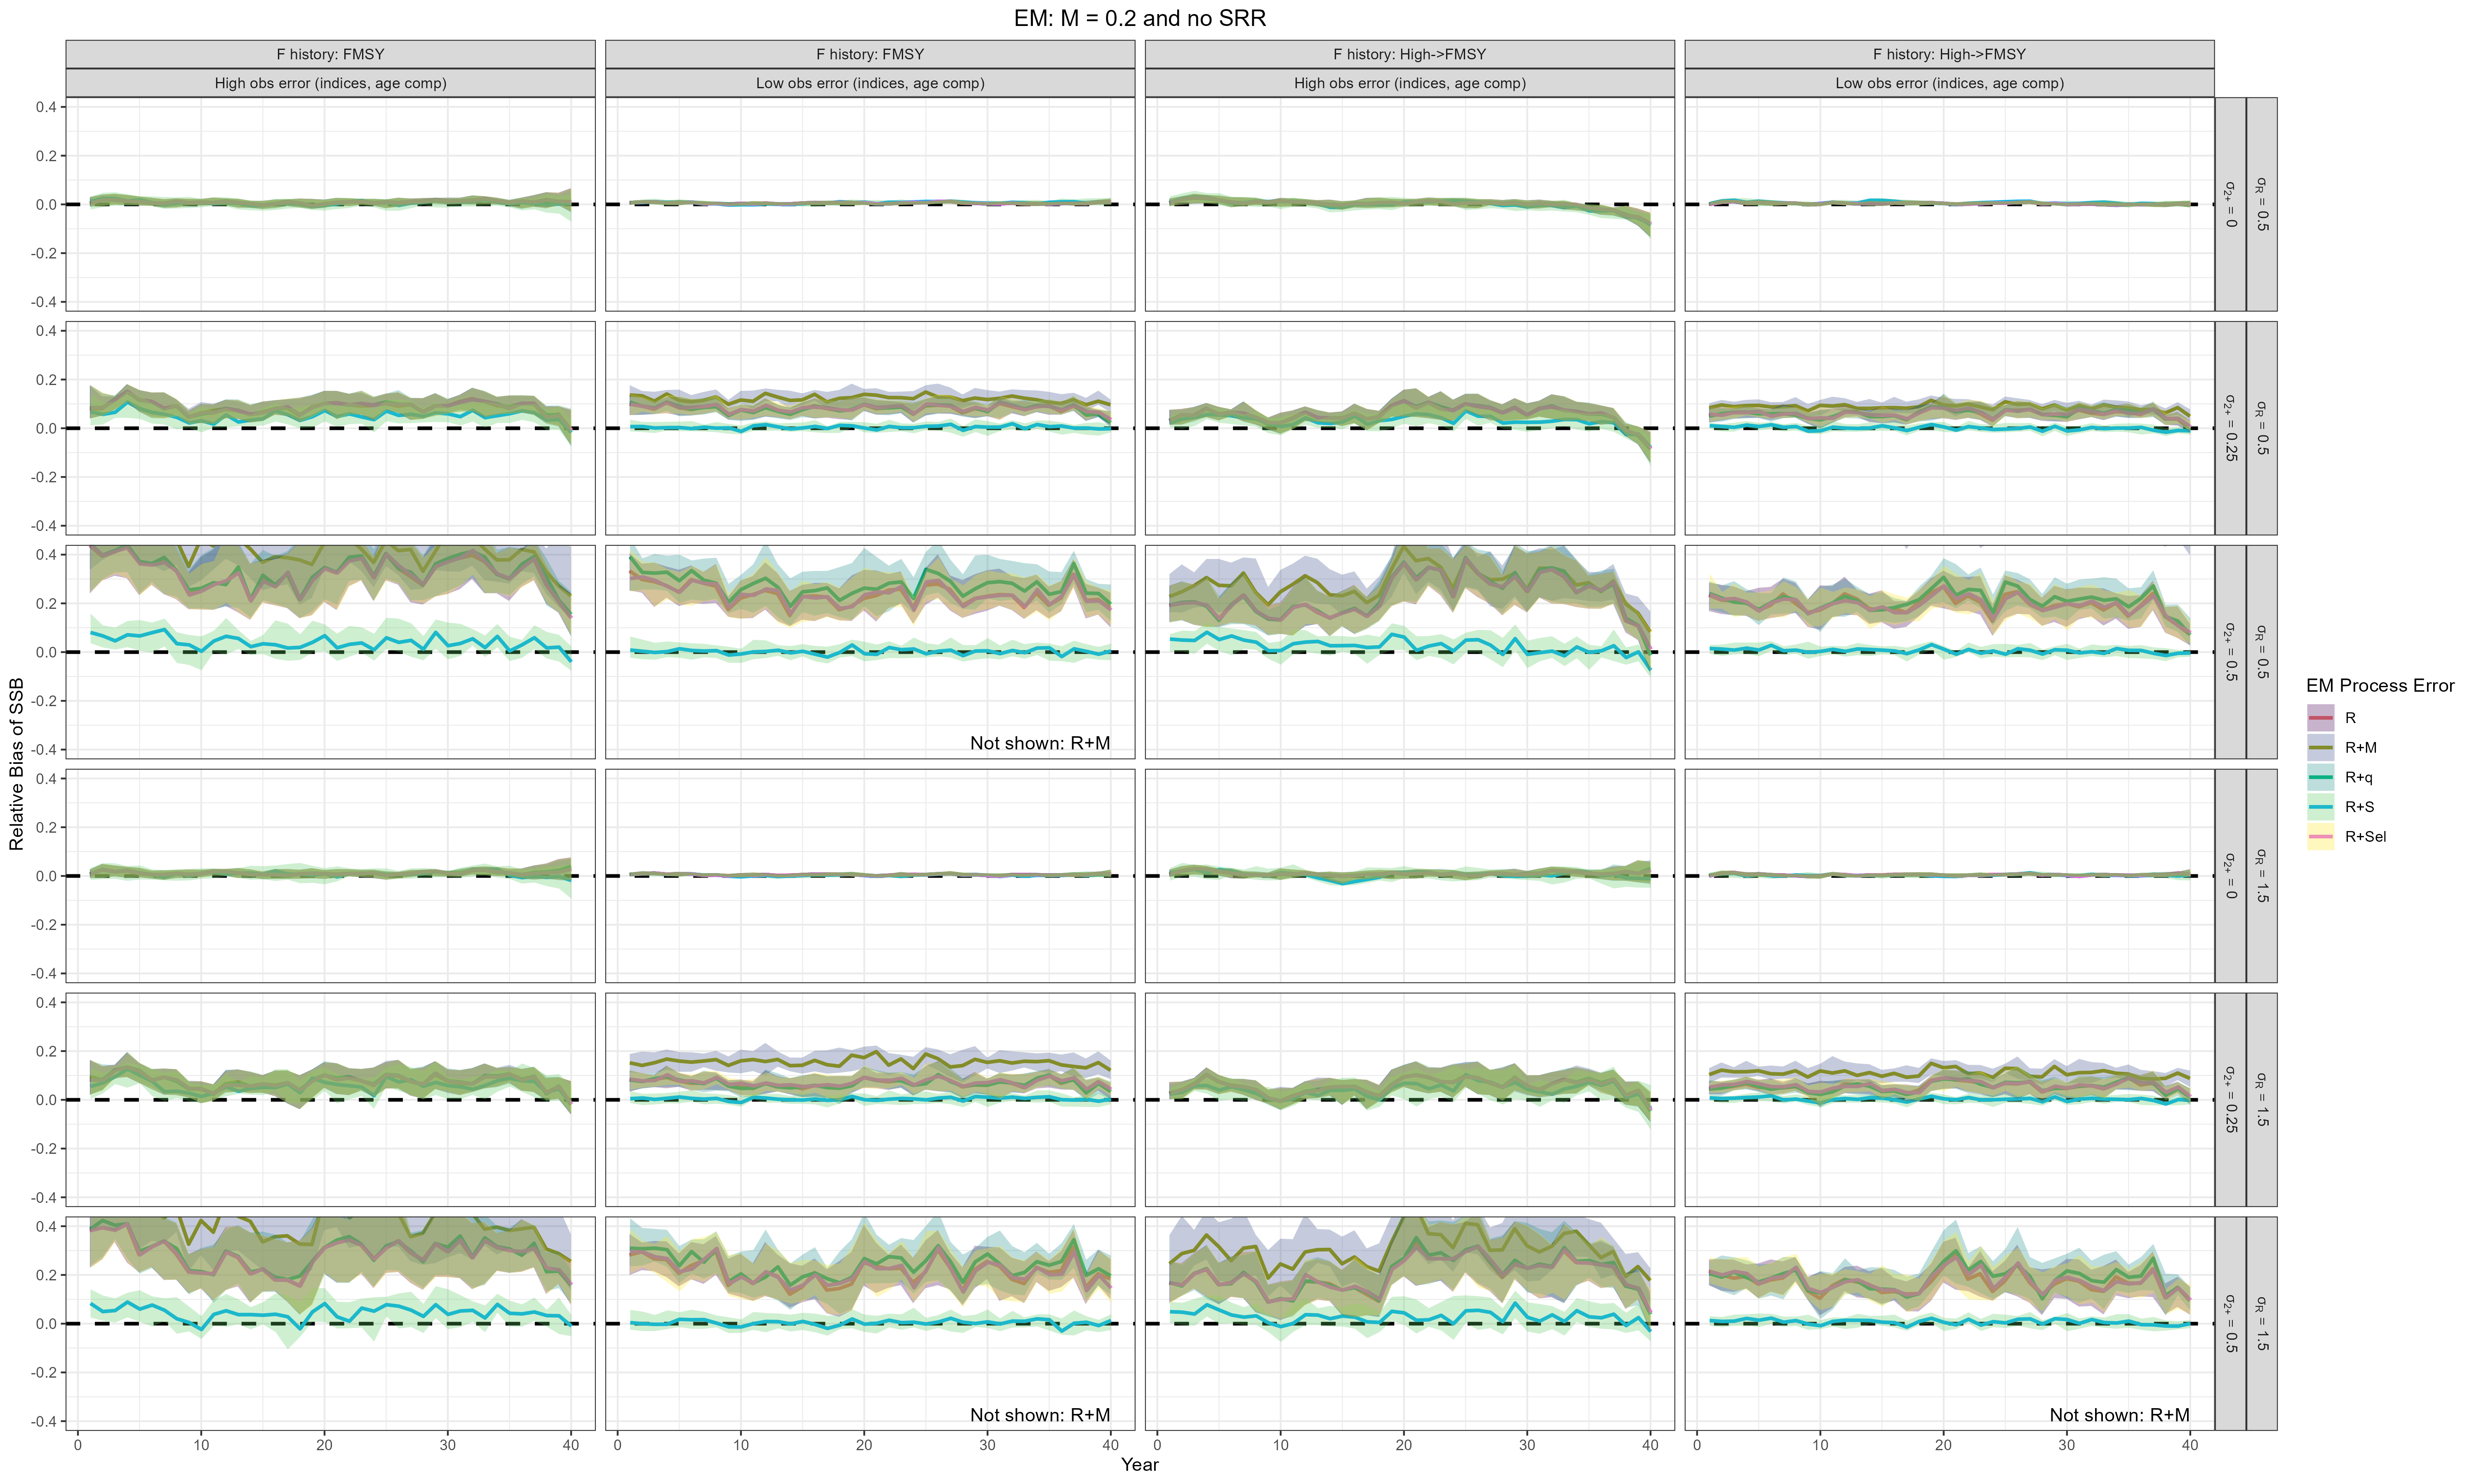
\includegraphics[width = \textwidth]{naa_om_R_MF_relbias_ssb.png}
\end{center}
\end{figure}
\end{landscape}

\begin{landscape}
\begin{figure}
\caption{Median relative bias of for SSB for estimating models that estimate mean recruitment and M is estimated.}\label{naa_om_em_R_ME_relbias_ssb}
\begin{center}
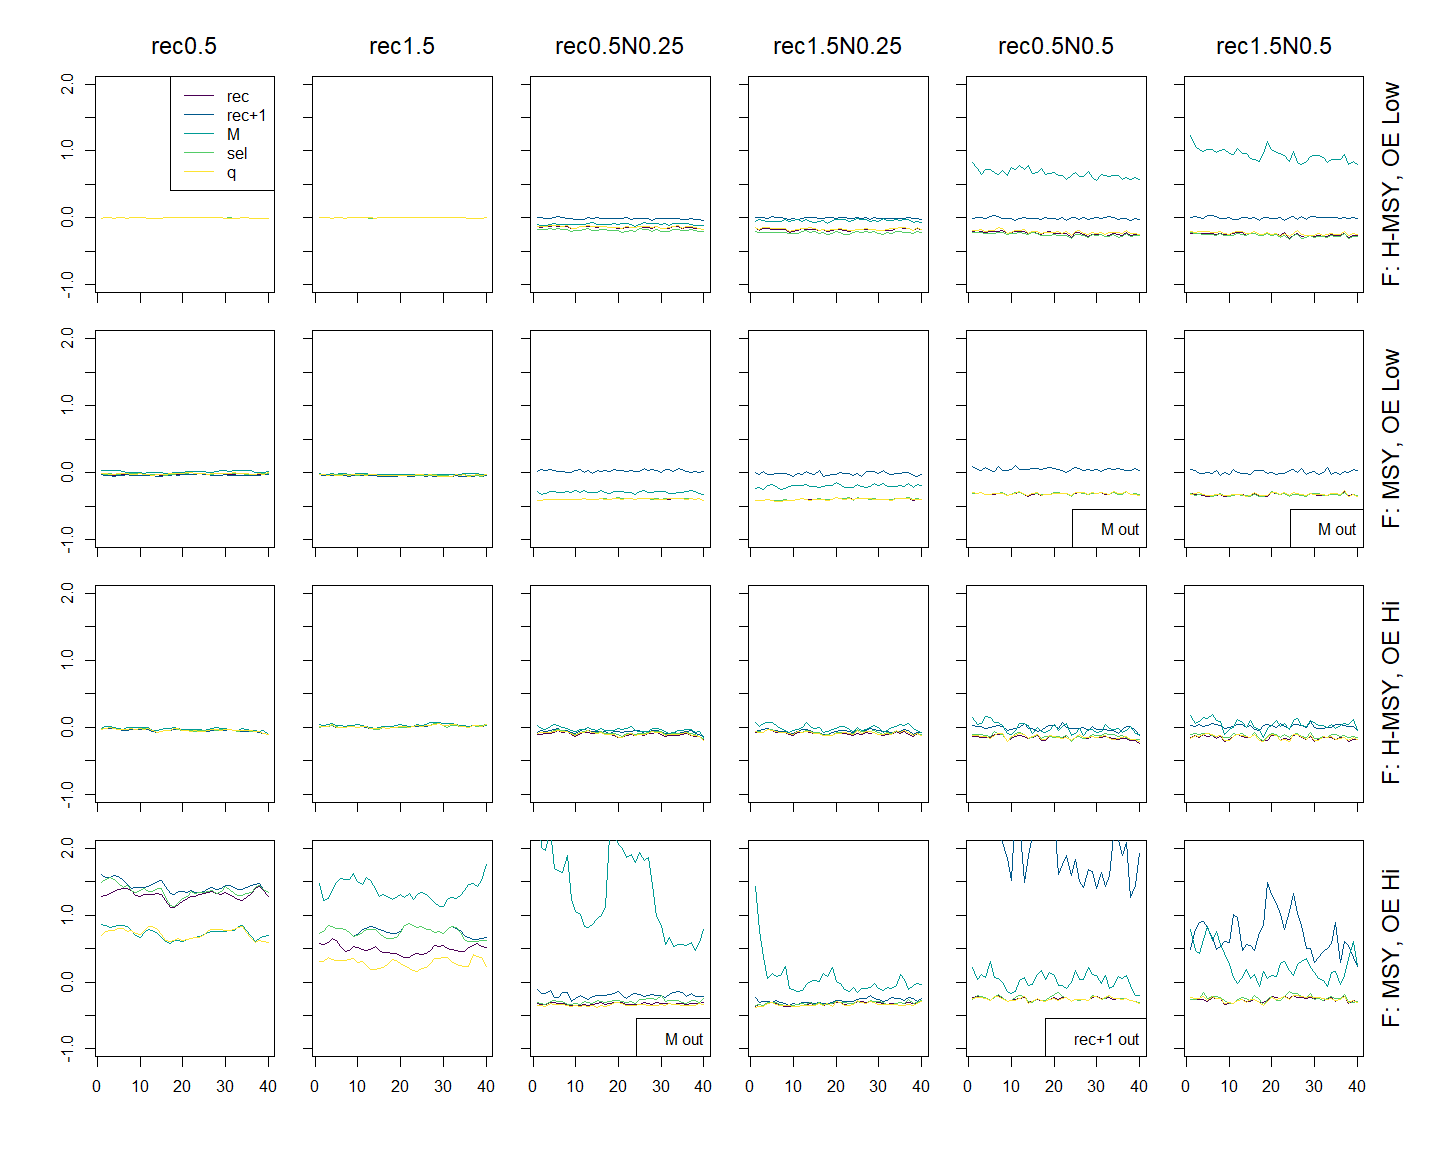
\includegraphics[width = \textwidth]{naa_om_R_ME_relbias_ssb.png}
\end{center}
\end{figure}
\end{landscape}

\begin{landscape}
\begin{figure}
\caption{Median relative bias of for SSB for estimating models that estimates a BH stock-recruitment function and M is fixed at the true value.}\label{naa_om_em_SR_MF_relbias_ssb}
\begin{center}
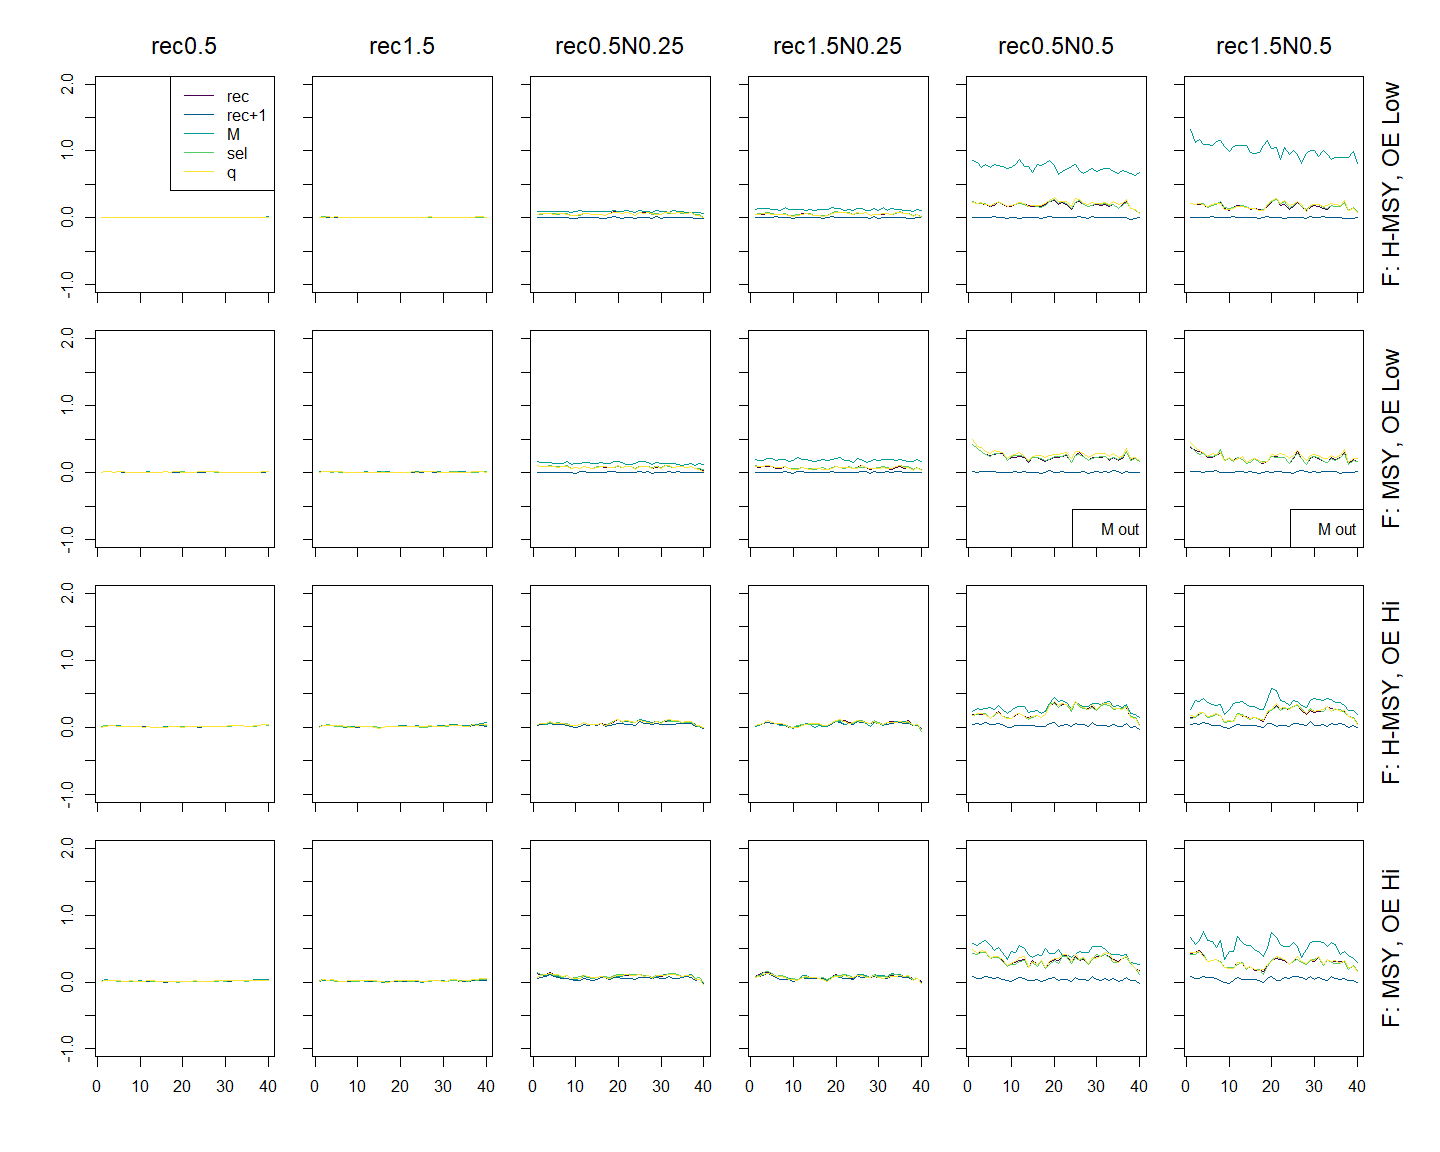
\includegraphics[width = \textwidth]{naa_om_SR_MF_relbias_ssb.png}
\end{center}
\end{figure}
\end{landscape}

\begin{landscape}
\begin{figure}
\caption{Median relative bias of for SSB for estimating models that estimates a BH stock-recruitment function and M is estimated.}\label{naa_om_em_SR_ME_relbias_ssb}
\begin{center}
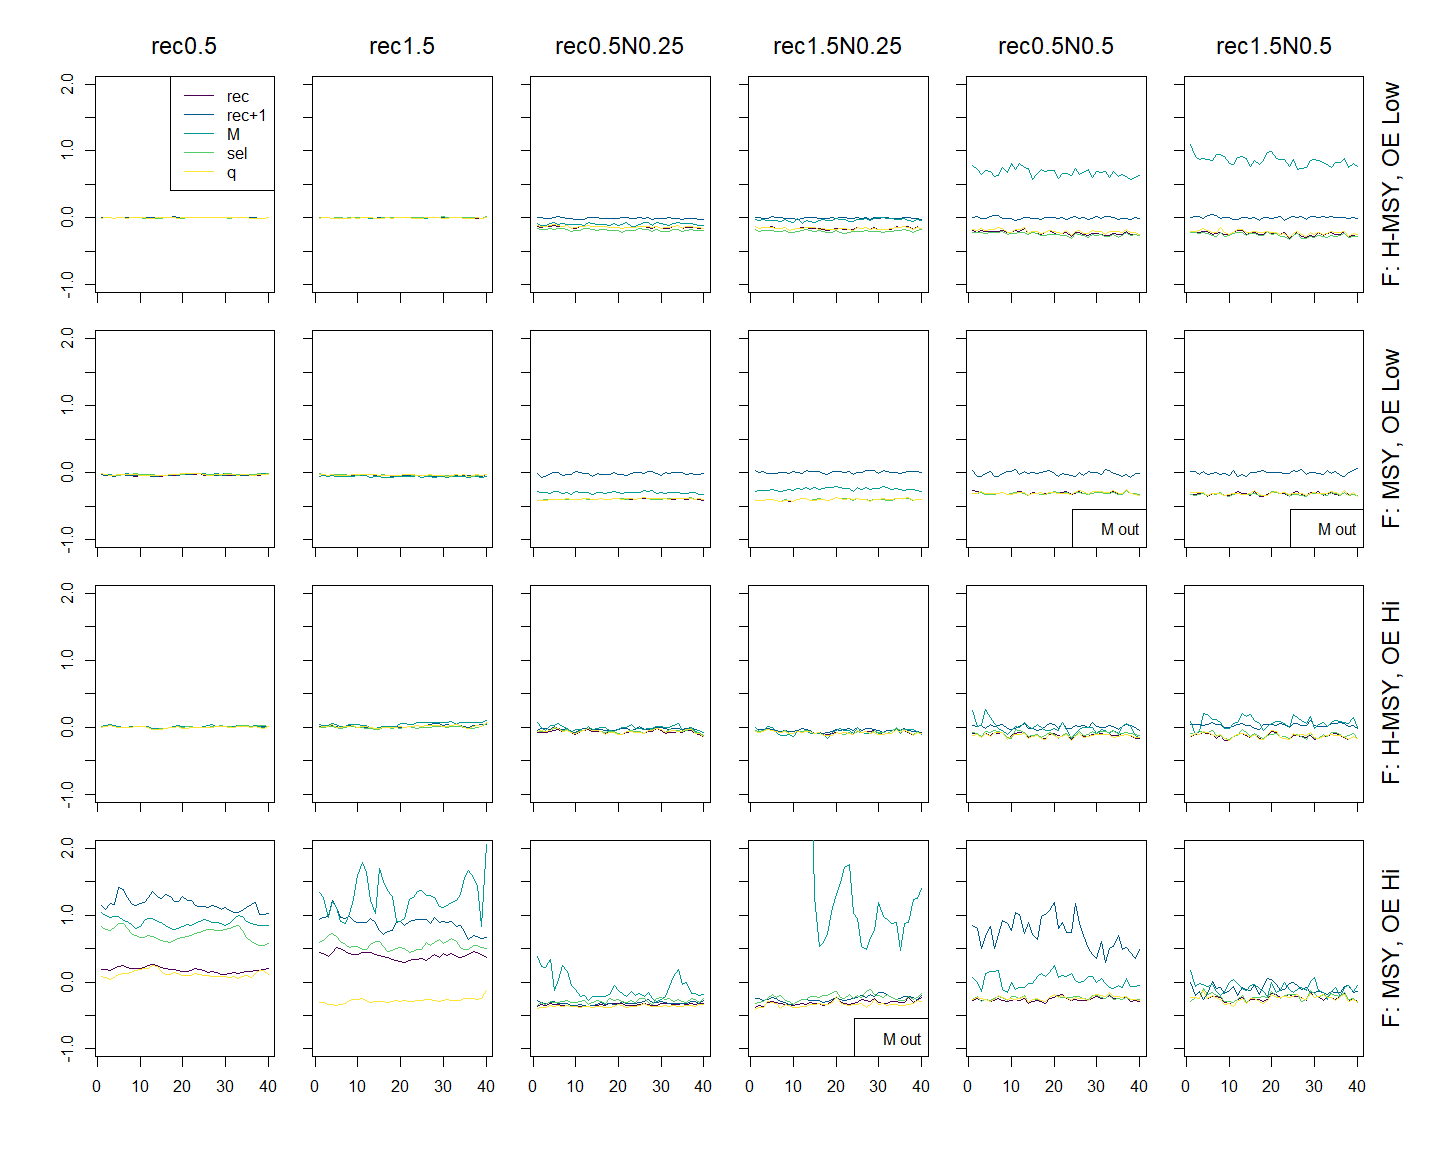
\includegraphics[width = \textwidth]{naa_om_SR_ME_relbias_ssb.png}
\end{center}
\end{figure}
\end{landscape}

\hypertarget{estimating-models-include-naa-random-effects-and-estimation-assumes-mean-r-or-bh-sr}{%
\subsubsection{Estimating models include NAA random effects and
estimation assumes mean R or BH
SR}\label{estimating-models-include-naa-random-effects-and-estimation-assumes-mean-r-or-bh-sr}}

\clearpage

\begin{table}
\caption{Operating models and estimation models all assume RE on recruitment only, estimating models assume mean recruitment or a B-H stock recruit relationship and M is fixed at the true value.}
{%latex.default(out, file = here("Project_0", "paper", "rec_om_em_R_SR_MF_aic_table.tex"),     table.env = FALSE, col.just = rep("r", dim(out)[2]), rowname = NULL)%
\begin{center}
\begin{tabular}{rrrrrr}
\hline\hline
\multicolumn{1}{c}{$\sigma_R$}&\multicolumn{1}{c}{$\sigma_N$}&\multicolumn{1}{c}{F-history}&\multicolumn{1}{c}{Obs Error}&\multicolumn{1}{c}{R only}&\multicolumn{1}{c}{BH}\tabularnewline
\hline
$0.5$&$$&H-MSY&L&$46$&$54$\tabularnewline
$1.5$&$$&H-MSY&L&$82$&$18$\tabularnewline
$0.5$&$$&MSY&L&$71$&$29$\tabularnewline
$1.5$&$$&MSY&L&$85$&$15$\tabularnewline
$0.5$&$$&H-MSY&H&$51$&$49$\tabularnewline
$1.5$&$$&H-MSY&H&$82$&$18$\tabularnewline
$0.5$&$$&MSY&H&$72$&$28$\tabularnewline
$1.5$&$$&MSY&H&$86$&$14$\tabularnewline
\hline
\end{tabular}\end{center}
}
\end{table}

\begin{table}
\caption{Operating models and estimation models all assume RE on recruitment only, estimating models assume mean recruitment or a B-H stock recruit relationship and M is estimated.}
{%latex.default(out, file = here("Project_0", "paper", "rec_om_em_R_SR_ME_aic_table.tex"),     table.env = FALSE, col.just = rep("r", dim(out)[2]), rowname = NULL)%
\begin{center}
\begin{tabular}{rrrrrr}
\hline\hline
\multicolumn{1}{c}{$\sigma_R$}&\multicolumn{1}{c}{$\sigma_N$}&\multicolumn{1}{c}{F-history}&\multicolumn{1}{c}{Obs Error}&\multicolumn{1}{c}{R only}&\multicolumn{1}{c}{BH}\tabularnewline
\hline
$0.5$&$$&H-MSY&L&$45$&$55$\tabularnewline
$1.5$&$$&H-MSY&L&$82$&$18$\tabularnewline
$0.5$&$$&MSY&L&$70$&$30$\tabularnewline
$1.5$&$$&MSY&L&$87$&$13$\tabularnewline
$0.5$&$$&H-MSY&H&$56$&$44$\tabularnewline
$1.5$&$$&H-MSY&H&$82$&$18$\tabularnewline
$0.5$&$$&MSY&H&$75$&$25$\tabularnewline
$1.5$&$$&MSY&H&$84$&$16$\tabularnewline
\hline
\end{tabular}\end{center}
}
\end{table}

\begin{table}
\caption{Operating models and estimation models all assume RE on all abundances at age, estimating models assume mean recruitment or a B-H stock recruit relationship and M is fixed at the true value.}
{%latex.default(out, file = here("Project_0", "paper", "naa_om_em_R_SR_MF_aic_table.tex"),     table.env = FALSE, col.just = rep("r", dim(out)[2]), rowname = NULL)%
\begin{center}
\begin{tabular}{rrrrrr}
\hline\hline
\multicolumn{1}{c}{$\sigma_R$}&\multicolumn{1}{c}{$\sigma_N$}&\multicolumn{1}{c}{F-history}&\multicolumn{1}{c}{Obs Error}&\multicolumn{1}{c}{R only}&\multicolumn{1}{c}{BH}\tabularnewline
\hline
$0.5$&$0.25$&H-MSY&L&$43$&$57$\tabularnewline
$1.5$&$0.25$&H-MSY&L&$84$&$16$\tabularnewline
$0.5$&$0.50$&H-MSY&L&$33$&$67$\tabularnewline
$1.5$&$0.50$&H-MSY&L&$77$&$23$\tabularnewline
$0.5$&$0.25$&MSY&L&$69$&$31$\tabularnewline
$1.5$&$0.25$&MSY&L&$88$&$12$\tabularnewline
$0.5$&$0.50$&MSY&L&$55$&$45$\tabularnewline
$1.5$&$0.50$&MSY&L&$87$&$13$\tabularnewline
$0.5$&$0.25$&H-MSY&H&$57$&$43$\tabularnewline
$1.5$&$0.25$&H-MSY&H&$84$&$16$\tabularnewline
$0.5$&$0.50$&H-MSY&H&$66$&$34$\tabularnewline
$1.5$&$0.50$&H-MSY&H&$79$&$21$\tabularnewline
$0.5$&$0.25$&MSY&H&$78$&$22$\tabularnewline
$1.5$&$0.25$&MSY&H&$88$&$12$\tabularnewline
$0.5$&$0.50$&MSY&H&$73$&$27$\tabularnewline
$1.5$&$0.50$&MSY&H&$83$&$17$\tabularnewline
\hline
\end{tabular}\end{center}
}
\end{table}

\begin{table}
\caption{Operating models and estimation models all assume RE on all abundances at age, estimating models assume mean recruitment or a B-H stock recruit relationship and M is estimated.}
{%latex.default(out, file = here("Project_0", "paper", "naa_om_em_R_SR_ME_aic_table.tex"),     table.env = FALSE, col.just = rep("r", dim(out)[2]), rowname = NULL)%
\begin{center}
\begin{tabular}{rrrrrr}
\hline\hline
\multicolumn{1}{c}{$\sigma_R$}&\multicolumn{1}{c}{$\sigma_N$}&\multicolumn{1}{c}{F-history}&\multicolumn{1}{c}{Obs Error}&\multicolumn{1}{c}{R only}&\multicolumn{1}{c}{BH}\tabularnewline
\hline
$0.5$&$0.25$&H-MSY&L&$44$&$56$\tabularnewline
$1.5$&$0.25$&H-MSY&L&$84$&$16$\tabularnewline
$0.5$&$0.50$&H-MSY&L&$31$&$69$\tabularnewline
$1.5$&$0.50$&H-MSY&L&$80$&$20$\tabularnewline
$0.5$&$0.25$&MSY&L&$68$&$32$\tabularnewline
$1.5$&$0.25$&MSY&L&$88$&$12$\tabularnewline
$0.5$&$0.50$&MSY&L&$55$&$45$\tabularnewline
$1.5$&$0.50$&MSY&L&$86$&$14$\tabularnewline
$0.5$&$0.25$&H-MSY&H&$59$&$41$\tabularnewline
$1.5$&$0.25$&H-MSY&H&$81$&$19$\tabularnewline
$0.5$&$0.50$&H-MSY&H&$67$&$33$\tabularnewline
$1.5$&$0.50$&H-MSY&H&$80$&$20$\tabularnewline
$0.5$&$0.25$&MSY&H&$66$&$34$\tabularnewline
$1.5$&$0.25$&MSY&H&$74$&$26$\tabularnewline
$0.5$&$0.50$&MSY&H&$74$&$26$\tabularnewline
$1.5$&$0.50$&MSY&H&$87$&$13$\tabularnewline
\hline
\end{tabular}\end{center}
}
\end{table}
\clearpage

\hypertarget{discussion}{%
\section{Discussion}\label{discussion}}

The estimating models assumed variances of aggregate catch and index
observations was known. This approximation may be appropriate for
indices where we have a reliable estimate of uncertainty based on the
survey design (), but there may be better approaches for the aggregate
catch such as an informed prior on the standard errors with realistic
bounds.

\hypertarget{acknowledgements}{%
\section*{Acknowledgements}\label{acknowledgements}}
\addcontentsline{toc}{section}{Acknowledgements}

This work was funded by NOAA Fisheries Northeast Fisheries Science
Center.

\pagebreak

\bibliography{sweep-paper}

\hypertarget{refs}{}
\begin{CSLReferences}{0}{0}
\end{CSLReferences}

\pagebreak

\clearpage

\end{document}
